\documentclass[11pt]{article}

\usepackage[margin=2.35cm]{geometry}
\usepackage{amsmath,amssymb,booktabs,array}
\usepackage{graphicx,xcolor,caption,enumitem}
\usepackage[hidelinks]{hyperref}
\usepackage{tikz}
\usetikzlibrary{arrows.meta,positioning}

\graphicspath{{figures/}}
\setlist[itemize]{topsep=3pt,itemsep=2pt,leftmargin=1.3em}
\setlist[enumerate]{topsep=3pt,itemsep=2pt,leftmargin=1.4em}
\captionsetup{font=small,labelfont=bf,skip=6pt}
\setlength{\parskip}{5pt}
\setlength{\parindent}{0pt}

\definecolor{navy}{HTML}{1F4E79}
\definecolor{rule}{HTML}{D0D5DD}

\pagestyle{plain}
\newcommand{\modelid}{LA-V22}
\newcommand{\doctype}{Model Development Document}

\title{\textcolor{navy}{\doctype}\\[4pt]
\large List-aware automated valuation, version 22}
\author{Model identification: \modelid}
\date{6 November 2026}

\begin{document}
\maketitle
\thispagestyle{empty}

\begin{center}
\small
\begin{tabular}{@{}>{\bfseries}l p{11.2cm}@{}}
Track & List-aware sale-price valuation \\
Status & Development candidate, pending independent validation \\
Population & Synthetic Toronto listings, sales closed January 2021--May 2026 \\
Decision metric & Median absolute percentage error (MdAPE) on sold price \\
Performance claim & Walk-forward MdAPE \(4.28\%\), MAPE \(5.37\%\), median bias \(+0.90\%\) \\
Benchmark & List price on the same sales: MdAPE \(7.26\%\), MAPE \(8.09\%\), median bias \(+5.68\%\) \\
Source notebooks & \texttt{list\_aware\_eda.ipynb}, \texttt{list\_aware\_models.ipynb} \\
Submission code & \texttt{features.py}, \texttt{models.py}, \texttt{run.py} \\
Figure reproduction & \texttt{model-report/reproduce\_v22\_figures.py} \\
\end{tabular}
\end{center}

\vspace{4pt}
{\color{rule}\hrule}
\vspace{8pt}

\section*{How to read this document}

This is the development record for \modelid, the list-aware model that predicts the closing price of a home that is already on the market. It is written so that model validation and internal audit can see the problem, the data, the specification, the estimation choices, and the out-of-time evidence without opening the notebooks.

Two results are easy to mix up, and they are kept apart throughout.

\begin{itemize}
\item \textbf{Developmental score.} One fit on every sale that closed before December 2025, scored on the 10,069 sales that closed from December 2025 through May 2026. This is the window used to compare specifications. For \modelid{} it is MdAPE \(4.43\%\).
\item \textbf{Walk-forward score.} The same six months, but each month is predicted by a model fit only on sales that had already closed. This is the performance claim: MdAPE \(4.28\%\).
\end{itemize}

The walk-forward number is the one a validation team should sign against. The developmental number is the model-selection record. Segmented charts in this document come from a fresh developmental refit. That refit reproduced the notebook to the reported precision (MdAPE \(4.43\%\), MAPE \(5.53\%\), median signed error \(+1.49\%\)).

\tableofcontents
\newpage

\section{Purpose and intended use}
\label{sec:purpose}

\subsection{The decision}

A listed home already has an asking price. The remaining question is what it will close at. Buyers, lenders, and internal valuation desks use that closing price for bid guidance, collateral checks, and a comparison against the ask. \modelid{} answers that question with a point estimate of sold price.

The companion off-market problem --- valuing a home that has no asking price --- is a different model. List price is an input here. It is absent there. A list-aware error must not be quoted as an off-market error. On this book the asking price alone already has a correlation of \(0.986\) with the sold price, so a list-aware model looks much tighter than a model that has to discover the price level from attributes.

\subsection{What the model returns}

For each home the model returns one positive dollar amount,
\[
\hat Y_i = L_i \exp(\hat g_i),
\]
where \(L_i\) is the list price and \(\hat g_i\) is the model's prediction of the log close ratio \(\log(Y_i/L_i)\). There is no prediction interval, no probability of selling above the ask, and no recommended haircut. Use is limited to a point estimate of the closing price at the time the home is listed, using only fields that exist on a list-aware test row.

\subsection{Users and non-uses}

The intended user is an internal valuation or model-risk function that can see the listing. The specification is implemented as \texttt{ListAwareModel} in \texttt{models.py}. \texttt{run.py} fits it, runs the walk-forward, and writes the test-file submission. Section~\ref{sec:repro} is that path. \texttt{ListPriceBaseline} is still in the file and is not the model the pipeline calls.

The model is not an appraisal. It does not use an inspection, a condition grade, or a human override. It should not be used to value a home that has not been listed, and it should not be fed \texttt{days\_on\_market}, \texttt{sold\_price}, or the third-party AVM field. Those columns are known only after the fact, or they are missing from the list-aware test file.

\subsection{Performance claim, stated once}

On the 10,069 sales closed from December 2025 through May 2026, with each month scored by a refit that could not see that month:

\begin{center}
\begin{tabular}{lrrr}
\toprule
 & MdAPE & MAPE & Median signed error \\
\midrule
List price, same homes & 7.26\% & 8.09\% & \(+5.68\%\) \\
\modelid{} walk-forward & 4.28\% & 5.37\% & \(+0.90\%\) \\
\bottomrule
\end{tabular}
\end{center}

MdAPE falls by \(2.98\) percentage points relative to taking the ask as the forecast, a \(41\%\) reduction. The typical prediction is still about \(0.9\%\) above the realized sale. That residual bias is discussed in Section~\ref{sec:calibration} and is a condition of use, not a rounding error to be ignored.

\section{Conceptual soundness}
\label{sec:concept}

\subsection{Economic object}

A list price is the seller's quote. In a hedonic market the quote already bundles size, type, location, and the seller's reading of recent sales (Rosen, 1974, is the usual reference for a price that is a function of attributes; here the quote is observed, so the attributes do not have to carry the whole price). What is left is the close ratio
\[
R_i = \frac{Y_i}{L_i}.
\]
Over the full book the median of \(R\) is \(0.98\) (homes close \(2.0\%\) under the ask) and the mean is about \(1.00\). The standard deviation of the percentage gap is \(10.7\) points. About \(58\%\) of sales close under the ask and \(42\%\) close over it. The 10th and 90th percentiles of \(R\) are \(0.89\) and \(1.15\).

So the ask is a strong but biased quote. In the validation window the bias is larger than the long-run median: the list-price forecast sits \(5.7\%\) above the sold price. A model that only reprints \(L_i\) locks that bias in. A model of \(R_i\), or of \(g_i = \log R_i\), can apply a discount that depends on the month, the neighbourhood, the property type, and how aggressive the ask is relative to recent sales.

\subsection{Why a multiplicative gap, briefly}

Dollar error grows with the price level. Sold prices run from about \(\$173{,}000\) to \(\$30\) million, with skew \(5.04\). Log sold price has skew \(0.80\). Working in \(\log(Y/L)\) does two useful things at once.

\begin{enumerate}
\item A unit of error is a percent, which matches MdAPE more closely than a squared dollar error does.
\item The list price is the base. Attributes then explain deviations from the ask, which is the quantity the desk does not already know.
\end{enumerate}

An ordinary least-squares fit of \(\log Y\) on \(\log L\) and the size and location controls gives an elasticity on the ask of \(0.894\) and an \(R^2\) of \(0.966\) (Section~\ref{sec:ols}). The ask carries the level. The residual series is where the time variation, and then the tree, do their work.

\subsection{Why a tree, briefly}

The close ratio is not a single citywide constant. It moves through 2021--2026 (Figure~\ref{fig:monthly}), and it differs by community and by how rich the ask is per square foot. Those are interactions and thresholds. A gradient-boosted tree (Friedman, 2001) is an additive expansion
\[
F(x) = \sum_{m=1}^{M} \eta \, f_m(x),
\]
with each \(f_m\) a regression tree and \(\eta\) the learning rate. LightGBM (Ke et al., 2017) fits that expansion on the squared log-gap loss
\[
\sum_i \bigl(g_i - F(x_i)\bigr)^2
\]
and accepts categorical fields, including a community with 145 levels, without a hand-built set of dummies.

Squared error on \(g_i\) is a smooth proxy for percentage error. It is not MdAPE. MdAPE is a median and ignores the worst tail; squared log error penalizes large percentage misses. The training loss and the reported metric are aligned in direction and different in detail. That difference is accepted and disclosed. Because the loss is on the log gap, \(\exp(F(x))\) estimates a conditional median of a roughly log-scale residual, which is the functional a median percentage metric wants. No smearing correction is applied.

\subsection{Why the evidence has to be out of time}

Peer medians, community effects, and the market lag are all computed from other sales. A random row split lets those features see sales that had not happened yet. The resulting MdAPE is an in-sample compliment, and it will not survive contact with next month. The development rule is: every lookup, every category level, and every tree is built from sales that closed before the home being scored. Walk-forward validation is that rule applied one month at a time. It is specified in Section~\ref{sec:walk}.

\section{Data}
\label{sec:data}

\subsection{Source and population}

All records are synthetic. They were generated from a process calibrated to Toronto property-type levels, neighbourhood differences, and the 2021--2026 boom and correction. Names, streets, and coordinates do not line up with real maps. No external census, rates, or listing feed is joined. No real sale is in the file.

\begin{center}
\begin{tabular}{llrr}
\toprule
File & Role & Rows & Sale or list dates \\
\midrule
\texttt{listings} & Estimation and validation & 150{,}000 & Sold 1 Jan 2021 -- 31 May 2026 \\
\texttt{test\_list\_aware} & Unlabelled deployment book & 4{,}064 & Listed 24 Jul 2025 -- 28 Sep 2026 \\
\bottomrule
\end{tabular}
\end{center}

The earliest listing date on the training file is 19 February 2020, because some January 2021 sales were listed the year before. The test file has no sold price. It is not used to fit, tune, or score anything in this document.

Five columns exist only on \texttt{listings}: sold price, sale date, days on market, the third-party AVM estimate, and the date of that estimate. Sold price is the target. The other four are excluded from the feature set for the reasons in Section~\ref{sec:excluded}.

\subsection{Estimation and validation samples}

\begin{center}
\begin{tabular}{lrrl}
\toprule
Sample & Rows & Sold from & Sold through \\
\midrule
Developmental estimation & 139{,}931 & 1 Jan 2021 & 30 Nov 2025 \\
Developmental validation & 10{,}069 & 1 Dec 2025 & 31 May 2026 \\
\bottomrule
\end{tabular}
\end{center}

The inner slice used only to choose tree settings is July--November 2025, with that search fit on sales through June 2025. Those inner months are then put back into the developmental estimation sample when the chosen settings are refit. That is a reason to prefer the walk-forward number, which never scores a month the tree has seen.

\subsection{Book composition}

Six property types. On the estimation sample the shares are condo apartment \(51.1\%\), detached \(28.6\%\), semi-detached \(9.5\%\), condo townhouse \(6.8\%\), freehold townhouse \(3.4\%\), and co-op apartment \(0.5\%\). There are 5 municipalities, 145 communities, and 16 architectural styles.

Training sold-price summary: median \(\$856{,}650\), mean \(\$1{,}073{,}917\), maximum \(\$30{,}000{,}000\). Median list price on the training sales is \(\$859{,}700\). The unlabelled test book is a little cheaper (median list \(\$816{,}250\)) and a little larger (median floor area \(1{,}200\) square feet against \(1{,}142\)). That shift is a deployment risk. It is not measured as an error, because the test labels are held back.

\subsection{Fields available at listing}

\begin{center}
\small
\begin{tabular}{llp{6.6cm}}
\toprule
Group & Columns & Treatment \\
\midrule
Quote & list price, date listed & Log price; month enters the time features \\
Size & area, beds, baths, parking, garage & Area parsed to square feet; counts kept as integers \\
Lot & lot front, lot depth & Missing when there is no lot; see Section~\ref{sec:clean} \\
Structure & type, style & Categorical, levels frozen on the estimation sample \\
Place & municipality, community, lat, lon & Community is categorical; coordinates stay in degrees \\
Text & remarks & Tested and left out; Section~\ref{sec:excluded} \\
\bottomrule
\end{tabular}
\end{center}

\section{Data preparation}
\label{sec:clean}

No sale is dropped. Missingness is structural, and the preparation keeps a trace of it.

\subsection{Floor area}

\texttt{house\_area} is text. A single token such as \texttt{622} is that number. A range such as \texttt{900-1099} becomes the midpoint, \(999.5\). The flag \texttt{area\_is\_range} is \(1\) when the source was a range, so the tree can treat a midpoint as a coarser measurement. Square feet enter the model as \(\log S_i\). Skew falls from \(2.90\) to \(0.60\).

\subsection{Lot fields}

\texttt{lot\_front} and \texttt{lot\_depth} are missing together on \(58.2\%\) of training rows and \(53.0\%\) of test rows. The missingness is the property type: condo apartment, condo townhouse, and co-op apartment are \(100\%\) missing; detached, semi-detached, and freehold townhouse are \(0\%\) missing. Filling those holes with a typical house frontage would invent land the unit does not have.

The rule actually used:

\begin{itemize}
\item \texttt{lot\_missing} \(= 1\) when frontage is missing.
\item \texttt{log\_lot\_front} \(= \log(\text{frontage})\) when present, and \(0\) when missing. Zero is \(\log 1\), so the frontage slope is identified from homes that have a lot.
\item \texttt{lot\_depth} is \(0\) when missing. Depth skew is \(0.61\); the log skew is \(-0.38\), so depth stays in feet.
\item \texttt{lot\_area} is the product of the raw frontage and depth, and is missing when either is missing. LightGBM splits on missingness directly, so this product is not zero-filled.
\end{itemize}

\subsection{Counts, coordinates, and prices}

Bedrooms, washrooms, parking, and garage stay in their recorded units. Their skew comes from a pile of small integers, and parking and garage can be zero, where a log is undefined. Latitude and longitude stay in degrees. Their skew is \(0.28\) and \(0.37\). A degree of longitude is about \(0.72\) times a degree of latitude at this latitude; the tree can split the two axes separately, so they are not rescaled. Rotated coordinates and a \(k\)-means region label were tried later and did not earn a place (Section~\ref{sec:challengers}).

List price and sold price are logged. There is no winsorisation. The \(\$30\) million tail stays in the estimation sample. The log, the median metric, and a minimum of 20 rows in each leaf are what keep that tail from setting the fit.

\subsection{Transforms, as chosen from the skew}

\begin{center}
\begin{tabular}{lrrl}
\toprule
Column & Skew & Skew of log & Decision \\
\midrule
Sold price & 5.04 & 0.80 & Log. Inside the gap target. \\
List price & 5.07 & 0.82 & Log feature. \\
Square feet & 2.90 & 0.60 & Log feature. \\
Lot front & 1.19 & 0.02 & Log, plus a missing indicator. \\
Lot depth & 0.61 & \(-0.38\) & Leave in feet. \\
Washrooms, parking, garage & 1.2--1.7 & --- & Leave as counts. \\
Bedrooms & 0.37 & --- & Leave as a count. \\
Latitude, longitude & 0.28, 0.37 & --- & Leave in degrees. \\
\bottomrule
\end{tabular}
\end{center}

Medians and category levels that feed features are computed on the estimation sample only. The validation months do not enter a fill value.

\subsection{Fields examined and left out}
\label{sec:excluded}

\textbf{Days on market.} Skew \(4.22\), median \(12\) days, mean \(22\). It is known when the sale closes, not when the home is listed. Using it would leak the outcome path into the feature.

\textbf{Third-party AVM.} Present on \(99.1\%\) of training sales and on none of the test rows. The estimate date runs as far as 30 June 2027, after the last training sale, so a naive join would also leak future information. It is not a production input for this track.

\textbf{Listing remarks.} A TF--IDF of unigrams and bigrams, reduced to 20 singular vectors fit on training remarks only, explained \(11.1\%\) of the training word matrix. Adding those components to the numeric booster moved developmental MdAPE from \(4.83\%\) to \(4.85\%\). The text is on the test file, so it could have been shipped. It did not improve the error, and it is not in \modelid{}.

\section{Market facts that drive the specification}
\label{sec:market}

\subsection{The ask and the close}

\begin{figure}[ht]
\centering
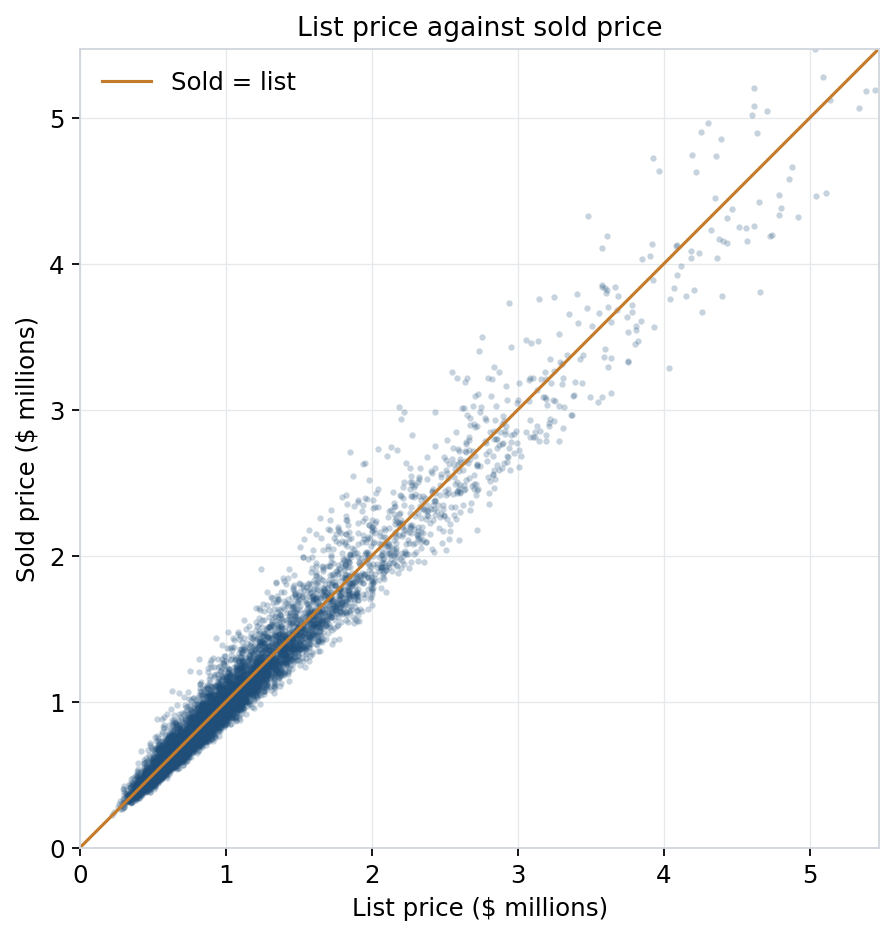
\includegraphics[width=0.72\linewidth]{list_vs_sold.png}
\caption{List price against sold price. A random sample of sales at or below the 99.5th percentile of either price (about \(\$5.47\) million). The line is a sale at the asking price. Correlation on the full book is \(0.986\).}
\label{fig:scatter}
\end{figure}

The cloud hugs the 45-degree line. That is why the benchmark of ``predict the list price'' is already a serious model, and why beating it by a few percentage points of MdAPE is the whole game. It is also why a regression on raw dollars can post an \(R^2\) of \(0.973\) and still be a weak valuation tool: most of that \(R^2\) is the ask.

\subsection{The close ratio moves}
\label{sec:stationarity}

\begin{figure}[ht]
\centering
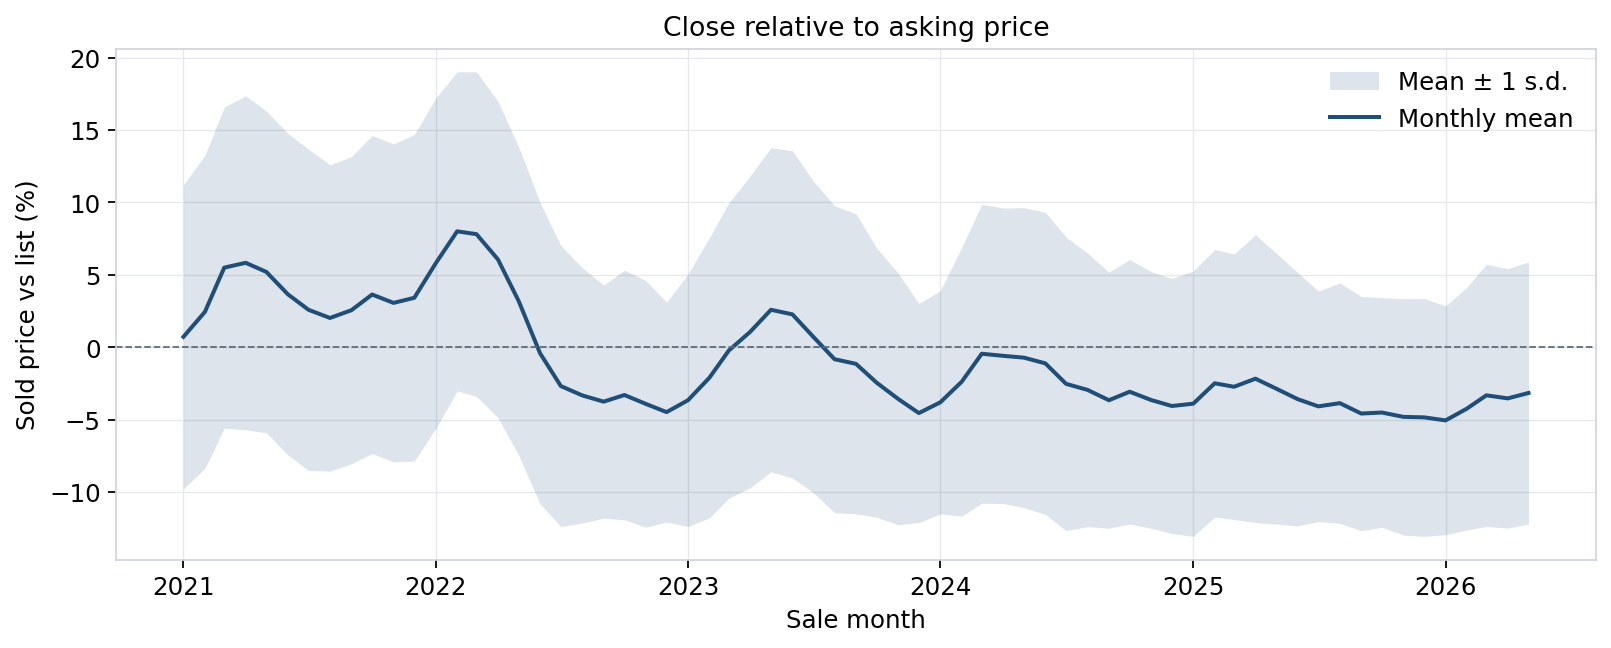
\includegraphics[width=\linewidth]{monthly_close_vs_list.png}
\caption{Percent by which the sold price exceeds the list price, averaged by sale month. The band is that month's mean plus and minus one standard deviation across homes. The validation window sits in a period of closes under the ask.}
\label{fig:monthly}
\end{figure}

The full-sample median gap is \(-2.0\%\). The validation-window list-price bias is \(+5.68\%\) (the ask is high relative to the close). A constant historical discount would be the wrong size for late 2025 and early 2026.

Two unit-root tests were run on the 65 monthly series, around a constant and around a linear trend.

\begin{center}
\small
\begin{tabular}{llcc l}
\toprule
Series & Specification & ADF \(p\) & KPSS \(p\) & Reading \\
\midrule
Median sold price & Constant & 0.580 & \(>0.10\) & Tests disagree \\
Median sold price & Linear trend & 0.033 & \(>0.10\) & Stationary around a trend \\
Median list price & Constant & 0.007 & \(>0.10\) & Stationary \\
Median list price & Linear trend & 0.175 & 0.024 & Not stationary \\
Mean \% above list & Constant & 0.025 & \(<0.01\) & Tests disagree \\
Mean \% above list & Linear trend & 0.001 & \(>0.10\) & Stationary around a trend \\
\bottomrule
\end{tabular}
\end{center}

The price level is not a fixed mean. The percent-above-list series is closer to stable once a trend is allowed, and it still drifts by more than a seasonal wiggle. A robust STL split gives seasonal strength \(0.80\) for median sold price (May high, January low, a swing of about \(\$144{,}000\) around the trend) and only \(0.15\) for the mean percent above list (a swing of \(4.4\) points). Calendar seasonality is mostly in the price level, which the ask already contains. The gap has a slow drift. That is why \modelid{} spends its time features on recent close ratios and on a residual forecast, and keeps month-of-year sine and cosine only as a small seasonal control.

\subsection{The log-linear residual and its forecast}
\label{sec:ols}

The developmental log-linear model is
\[
\log Y_i = \beta_0 + \beta_L \log L_i + z_i^\top\gamma + e_i,
\]
with \(z_i\) the numeric design of Section~\ref{sec:features}. On 139{,}931 sales, \(R^2 = 0.966\), \(\hat\beta_L = 0.894\) (standard error \(0.001\)), and residual skew \(0.72\). The same regression in raw dollars has residual skew \(2.56\). The log scale is the one a Gaussian working model can live with. Even so, Jarque--Bera still rejects at this sample size. The residual plots are used as a comparison of skew, not as a claim of exact normality.

The monthly mean of \(e_i\) is the series the time-series piece models. An augmented Dickey--Fuller test with a trend gives \(p = 0.0002\), so the series is not differenced. The fitted model on the 59 estimation months (January 2021 through November 2025) is a constant, a one-month autoregression, and a 12-month autoregression:
\[
\bar e_m = c + \phi \bar e_{m-1} + \Phi \bar e_{m-12} + u_m.
\]

\begin{center}
\begin{tabular}{lrrrr}
\toprule
Term & Estimate & Std.\ error & \(z\) & \(p\) \\
\midrule
Intercept & \(-0.0046\) & 0.002 & \(-2.54\) & 0.011 \\
AR(1) & 0.872 & 0.043 & 20.39 & \(<0.001\) \\
Seasonal AR(12) & 0.370 & 0.114 & 3.25 & 0.001 \\
Innovation variance & 0.0001 & --- & --- & --- \\
\bottomrule
\end{tabular}
\end{center}

In-sample \(R^2\) on this monthly series is \(0.885\). That number is a share of residual-month variance, not a share of home-price variance. The one-month coefficient near \(0.87\) says a soft month tends to be followed by another soft month. The forecast log residual for the validation months runs from \(-0.062\) in December 2025 to about \(-0.051\) in April 2026. A log residual of \(-0.054\) is a price level about \(5.3\%\) below the log-linear fit, which lines up with the \(5.7\%\) overstatement of the raw ask in that window.

A January--May 2022 pulse and a post-June 2022 level shift were added to this time-series model because the residual plot shows a spike in the first half of 2022. Conditional on the autoregression, both extra terms are indistinguishable from zero (pulse \(p = 0.89\), level shift \(p = 0.64\)). The developmental MdAPE moved from \(4.78\%\) to \(4.80\%\). The spike is already in the lagged residual. The pulse specification was not carried forward.

Adding the forecast residual back onto the log-linear prediction, the same shift for every home sold in a month, cuts developmental MdAPE from \(7.13\%\) (log-linear alone) to \(4.78\%\), and cuts median signed error from \(+5.95\%\) to \(+0.25\%\). Most of what is wrong with ``sold equals list'' in this window is a common, persistent discount. \modelid{} does not add that forecast on at the end. It passes the same information in as a feature, \texttt{list\_month\_factor}, and lets the tree decide how much of it to use given the rest of the home.

\section{Feature specification}
\label{sec:features}

The scored model has 23 inputs. Nothing in the design is computed from the home's own sold price, from a later sale, or from the unlabelled test file.

\subsection{Attribute block}

The numeric design, shared with the log-linear model, is \(\log L\), \(\log S\), the lot treatment of Section~\ref{sec:clean}, bedrooms, washrooms, parking, garage, latitude, and longitude. On top of that:

\begin{itemize}
\item \texttt{listed\_month\_sin} and \texttt{listed\_month\_cos}, from the listing month \(m \in \{1,\ldots,12\}\):
\[
\sin(2\pi m/12), \qquad \cos(2\pi m/12).
\]
Two columns so that December sits next to January.
\item \texttt{market\_lag}: the median of \(\log(Y/L)\) among estimation-sample sales in the calendar month before the listing month. Listing months after the last estimation month receive that last month's median, held flat, so the feature does not go missing at the edge of the sample.
\item \texttt{lot\_area} and \texttt{area\_is\_range}, as defined above.
\item Property type, architectural style, and municipality, as categoricals. Levels are the values seen in the estimation sample. An unseen level is missing, and LightGBM keeps the missing value rather than receiving an imputed label.
\end{itemize}

\subsection{Peer ask}

Peer ask measures whether this ask, per square foot, is rich or cheap against homes like it that have already sold.
\[
\text{peer ask}_i
= \frac{L_i / S_i}{m_{c(i),\,t(i)}(\tau_i)}.
\]
Here \(\tau_i\) is the listing month, \(c(i)\) the community, \(t(i)\) the property type, and \(m\) is the median sold price per square foot among sales that closed strictly before \(\tau_i\). The sale month of the home itself is not eligible, and neither is any sale that had not closed by the listing month.

If fewer than 30 such sales exist for that community and type, \(m\) falls back to the type-level median. Thirty is a stability floor, not a tuned hyperparameter: a median of a handful of sales is a noisy feature. On the developmental estimation sample the community median is used for \(84\%\) of rows. On the validation rows, whose listings can look back across the whole estimation history, it is used for \(97\%\).

A value above 1 means the ask per square foot is above the historical local sold price per square foot. Those homes should close further under the ask if sellers have overreached, and the tree is free to learn the opposite if a high peer ask instead marks homes that start bidding wars. The gain chart says the column is the most used split in the model (Section~\ref{sec:gain}).

\subsection{Recent community discount}

The peer median is a long history. Bargaining also has a short memory. The recent discount is the median of \(Y/L\) for the same community and type over the three sale months before the listing month. The same floor of 30 sales applies. Failing that, the feature falls back to the property-type median over the same three months, and failing that it is left missing.

Coverage is much thinner than for peer ask, because three months is a small cell:

\begin{center}
\begin{tabular}{lccc}
\toprule
 & Community cell & Type fallback & Missing \\
\midrule
Estimation sample & 41\% & 55\% & 3\% \\
Developmental validation & 15\% & 39\% & 46\% \\
\bottomrule
\end{tabular}
\end{center}

On a single fit that stops in November 2025, almost half of the validation rows do not get a local three-month median. The type fallback and the community category have to carry those rows. Under walk-forward the tables are rebuilt every month, so the window slides forward with the market. That is one reason the walk-forward bias (\(+0.90\%\)) is smaller than the developmental bias (\(+1.49\%\)).

\subsection{Listing-month factor}

This is the upstream residual forecast of Section~\ref{sec:ols}, attached to the listing month. If the listing month lies in the forecast horizon, the feature is the forecast \(\hat{\bar e}\). If the listing month is earlier, the feature is the realized mean log residual of the previous month. The median value on the developmental validation rows is \(-0.0539\).

It is a citywide, smoothed measure of how far recent closes have sat from the attribute-adjusted ask. It is not the same object as \texttt{market\_lag} (a one-month raw median of \(\log(Y/L)\)) or as the recent discount (a local three-month median of \(Y/L\)). All three survive in the gain ranking, which is the empirical case that they are not copies of one another.

\subsection{Community as a category}

\modelid{} adds the community name to the categorical set, with levels frozen on the estimation sample. Every validation community in the developmental split had been seen in estimation (unseen share \(0\%\)). A new community at deployment would be missing and would fall back on type, municipality, coordinates, and the peer features.

The category is a persistent neighbourhood intercept: some communities close systematically tight or loose relative to what size, type, and the ask imply. The three-month discount is the current bargaining climate. One can be calm while the other is not. Walk-forward is what justifies keeping both. Adding the category improved every one of the six months (Section~\ref{sec:walk}).

\subsection{What the splits actually use}
\label{sec:gain}

\begin{figure}[ht]
\centering
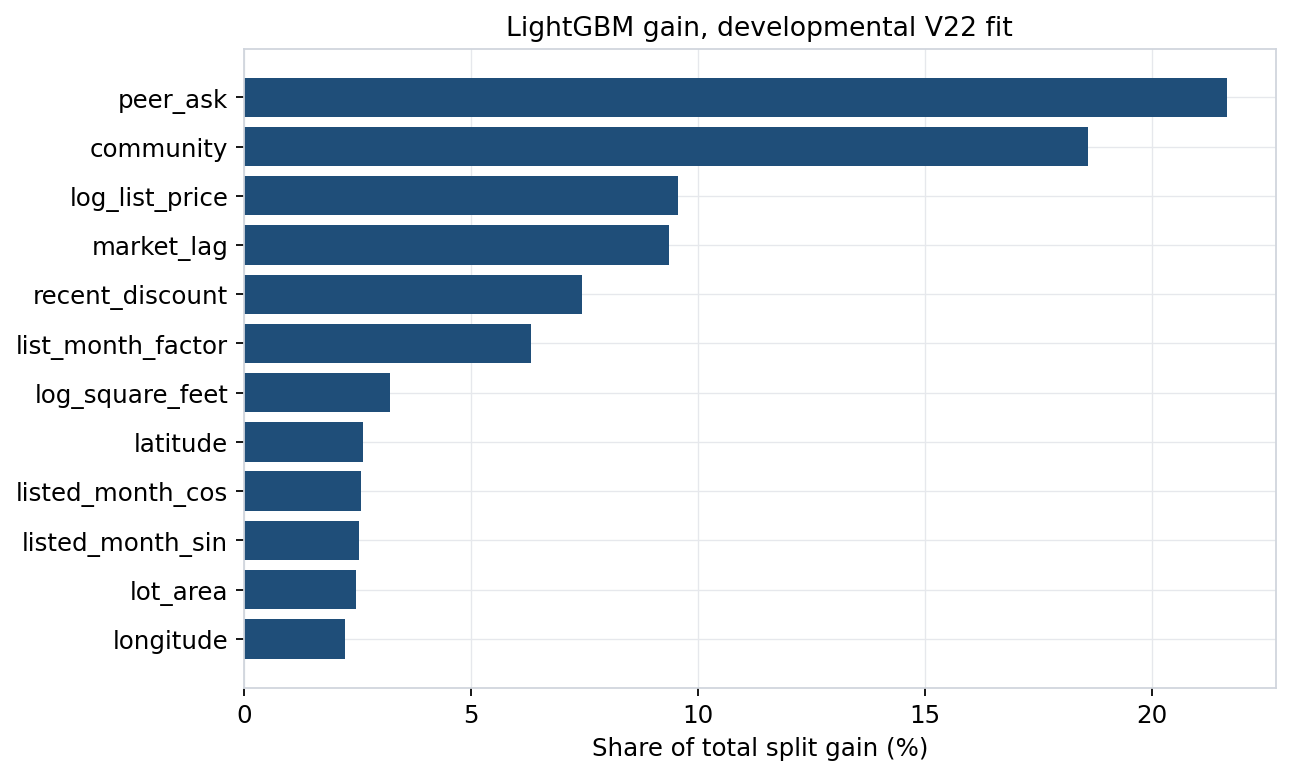
\includegraphics[width=0.92\linewidth]{feature_gain.png}
\caption{Share of total LightGBM split gain on the developmental \modelid{} fit. Gain is an in-sample description of the fitted tree. It is not a causal importance and it is not a promise about a shuffled-column test.}
\label{fig:gain}
\end{figure}

\begin{center}
\begin{tabular}{lr l}
\toprule
Feature & Gain share & Reading \\
\midrule
\texttt{peer\_ask} & 21.6\% & Richness of the ask against local sold \$/sqft \\
\texttt{community} & 18.6\% & Persistent neighbourhood close pattern \\
\texttt{log\_list\_price} & 9.6\% & The gap itself depends on the price level \\
\texttt{market\_lag} & 9.4\% & Citywide close ratio in the prior month \\
\texttt{recent\_discount} & 7.5\% & Local three-month bargaining climate \\
\texttt{list\_month\_factor} & 6.3\% & Smoothed residual forecast \\
\texttt{log\_square\_feet} & 3.2\% & Size given the ask \\
Coordinates, month, lot area & about 2--3\% each & Secondary \\
\bottomrule
\end{tabular}
\end{center}

Municipality is \(0.05\%\) of gain and the lot-missing flag is \(0.07\%\). Both are nearly redundant once community and property type are present. They are retained because they are the coarse fallback when a community is unseen, and because removing them was not an isolated test of the final specification. Their near-zero gain is a reason not to tell a story in which municipality is a driver.

An earlier permutation check, on a numeric booster that predicted log price rather than the log gap, attributed \(35.9\) points of MdAPE to \(\log L\) and less than \(1\) point to any other single column. That result belongs to a different target. Once the ask is the base rather than the thing being predicted, \(\log L\) is no longer the dominant split, and peer ask and community are. Both facts are consistent. The ask sets the level; the model of the gap spends its capacity on whether that ask will hold.

\subsection{Feature decisions that were tested and not kept}

\begin{center}
\small
\begin{tabular}{p{4.2cm}p{9.2cm}}
\toprule
Candidate & What happened \\
\midrule
Remarks, 20 SVD components & Developmental MdAPE \(4.85\%\) against \(4.83\%\) without them. \\
Cumulative type-level sold-to-list median (V10) & Outer-window XGBoost MdAPE worsened from \(4.53\%\) to \(4.63\%\). The short-window discount above is a different feature and was kept. \\
Rotated coordinates, \(k\)-means regions, 10 nearest past sales & Developmental MdAPE \(4.52\)--\(4.53\%\), no improvement on the LightGBM they were added to. \\
A 2022 pulse in the residual model & Coefficients insignificant. MdAPE \(4.80\%\) against \(4.78\%\). \\
\bottomrule
\end{tabular}
\end{center}

One disagreement in the record should be explicit. On an inner XGBoost comparison (fit through June 2025, scored July--November 2025) the feature set that included the cumulative type discount and the listing-month factor had the best inner MdAPE, \(4.542\%\), and peer ask alone had the worst, \(4.707\%\). On the December--May window the ranking flipped. The LightGBM line that became \modelid{} was built on peer ask plus the listing-month factor, which is the set that held up out of that inner slice, and the cumulative type discount was not carried forward. Inner-window feature ranks are a screen. They are not the adoption decision.

\section{Estimation and calibration}
\label{sec:calibration}

\subsection{The fitted equation}

\[
\hat g_i = F_{\hat\theta}(x_i), \qquad \hat Y_i = L_i \exp(\hat g_i),
\]
where \(F\) is a LightGBM regressor and \(x_i\) is the 23-column design. Categorical inputs are type, style, municipality, and community.

\subsection{Settings}

Settings were chosen by a grid on the V9 column set (attributes plus peer ask), fit through June 2025 and scored on July--November 2025 by inner MdAPE. The grid covered leaves in \(\{31, 63, 127, 255\}\), learning rates in \(\{0.03, 0.05, 0.10\}\), and 300 to 700 trees. The selected point, and the fixed settings around it:

\begin{center}
\begin{tabular}{ll}
\toprule
Setting & Value \\
\midrule
Number of leaves & 127 \\
Learning rate & 0.03 \\
Number of trees & 700 \\
Minimum rows in a leaf & 20 \\
Row subsample & 0.8, every tree \\
Column subsample & 0.8 \\
L2 penalty on leaf weights & 1.0 \\
Random seed & 0 \\
Objective & Squared error on \(\log(Y/L)\) \\
\bottomrule
\end{tabular}
\end{center}

The inner scores were flat. The winner was inner MdAPE \(4.620\). The next three settings sat at \(4.649\), \(4.660\), and \(4.670\). The adopted point is the conservative end of a plateau: a smaller learning rate and more trees, not a deeper tree that won by a tenth of a point and might not travel.

These settings were not re-searched after the target changed from \(\log Y\) to \(\log(Y/L)\), and they were not re-searched after community was added. Re-opening the grid on the same inner months would have spent that slice twice. The walk-forward result is therefore the result of a specification that was not re-optimised for its final target. That is the more honest number to carry.

\subsection{Other boosters}

On a common early feature set, XGBoost (depth 8, learning rate \(0.05\), 400 trees) reached developmental MdAPE \(4.69\%\), CatBoost \(4.81\%\), and a random forest \(5.05\%\). LightGBM at the settings above, once peer ask was in the design, matched the better XGBoost numbers and handles the community category without a dummy expansion. That is the practical reason it is the engine. There is no claim that LightGBM is the unique consistent estimator of a close ratio.

\subsection{Retransformation}

The tree targets \(g = \log(Y/L)\). Exponentiating and multiplying by \(L\) returns a price. If the error in \(g\) is roughly symmetric, this is a median forecast of \(Y\), not a mean forecast. MdAPE and the median signed error are median functionals, so the match is deliberate. A mean-unbiased smearing factor would chase a different decision metric than the one this model is judged on.

\subsection{Empirical calibration of the close ratio}

\begin{figure}[ht]
\centering
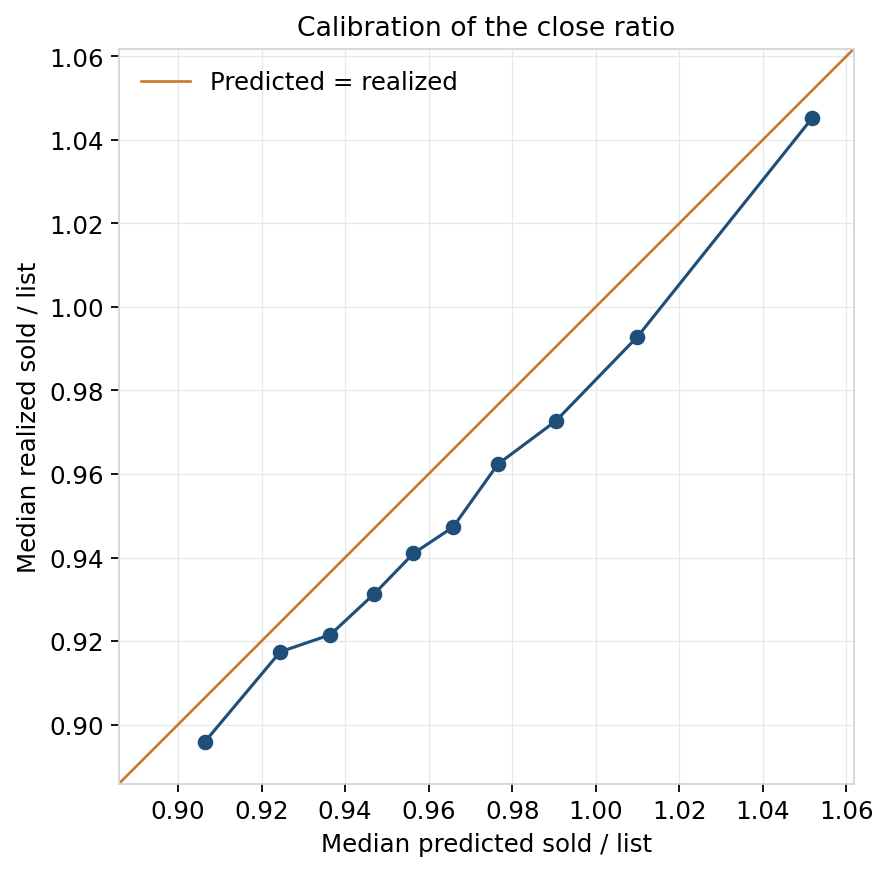
\includegraphics[width=0.62\linewidth]{calibration_ratio.png}
\caption{Developmental validation. Homes are grouped into ten bins of predicted close ratio. Each point is the median prediction in the bin against the median realized ratio. The line is agreement.}
\label{fig:cal}
\end{figure}

The bins rise together: a higher predicted ratio is a higher realized ratio, from about \(0.90\) up to about \(1.05\). The curve lies below the diagonal across the range. The model orders homes correctly and sits high, by roughly one to one and a half percentage points of the close ratio. That is the same fact as the developmental median signed error of \(+1.49\%\).

A final scalar haircut was the obvious repair. Two versions were tested. One multiplies the tree price by \(\exp(w \times \text{listing-month factor})\), with \(w\) chosen on a prior inner window. The other subtracts a recent median log residual (the V19 level shift). Both improve a single six-month fit and then fail to dominate under walk-forward, where the haircut is re-estimated without seeing the scored month (Section~\ref{sec:challengers}). V15's walk-forward median signed error is \(-1.75\%\): the haircut overshoots. \modelid{} does not apply one. The remaining \(+0.90\%\) walk-forward bias is reported as a known level error.

A partial reason the bias survives is mechanical. The listing-month factor on the validation rows is about \(-0.054\), and a full pass-through would cut prices by about \(5\%\), which is the size of the ask's own bias. The tree's gain share on that column is \(6.3\%\). It uses the information. It does not treat it as a mandatory citywide multiplier, because the right pass-through depends on the home. Forcing the multiplier was the experiment that overshot.

\subsection{Where a constant bias is not constant}

On the developmental fit, median signed error is \(+3.69\%\) in the cheapest sold-price decile (sold price up to about \(\$440{,}000\)) and near zero or slightly negative in the ninth decile. Co-op apartments, with 48 validation sales, have median signed error \(+3.6\%\). A single citywide bias number understates the cheap end of the book. Section~\ref{sec:errors} has the table. Monitoring should look at the low-price band separately.

\section{Architecture}
\label{sec:architecture}

\modelid{} is one tree model with two upstream constructions. It is not a stack of successive price forecasts added together. The OLS and the SARIMAX exist to build \texttt{list\_month\_factor}. The lookup tables exist to build peer ask and the recent discount. LightGBM then fits the log gap, and the list price scales the result back to dollars.

\begin{figure}[ht]
\centering
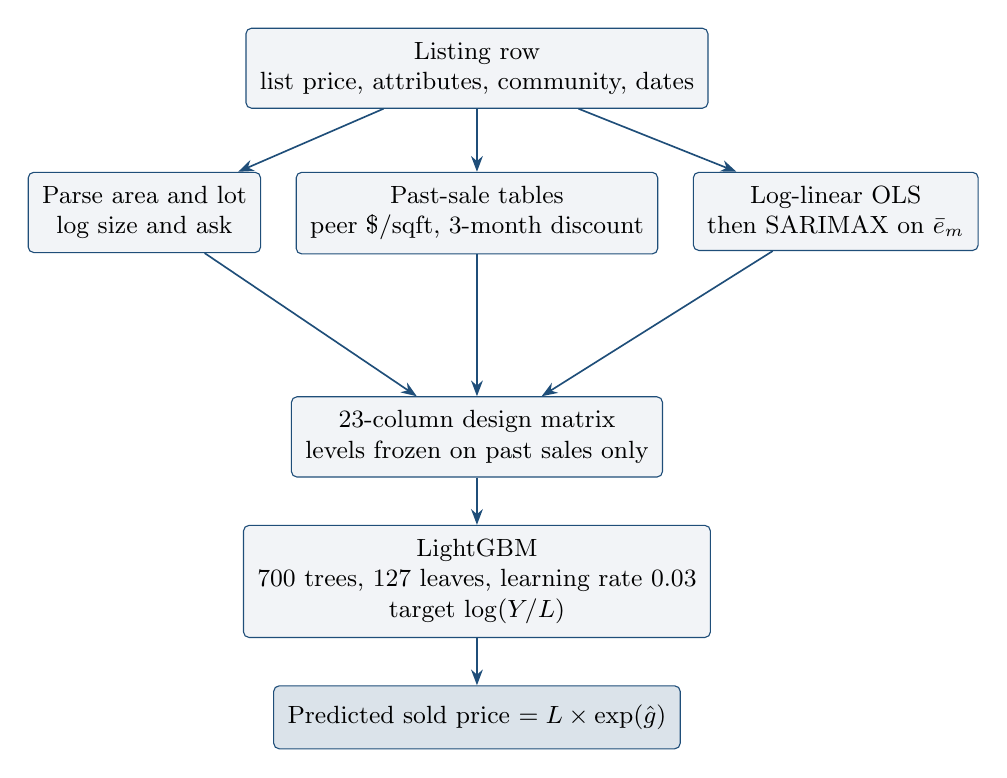
\begin{tikzpicture}[
  font=\small,
  box/.style={draw=navy, rounded corners=2pt, align=center, inner sep=5pt,
              minimum height=8mm, fill=navy!6},
  arr/.style={-{Stealth[length=2mm]}, semithick, draw=navy}
]
\node[box] (raw) {Listing row\\ list price, attributes, community, dates};
\node[box, below left=8mm and -2mm of raw] (attr) {Parse area and lot\\ log size and ask};
\node[box, below=8mm of raw] (tables) {Past-sale tables\\ peer \$/sqft, 3-month discount};
\node[box, below right=8mm and -2mm of raw] (ts) {Log-linear OLS\\ then SARIMAX on \(\bar e_m\)};
\node[box, below=18mm of tables] (design) {23-column design matrix\\ levels frozen on past sales only};
\node[box, below=6mm of design] (lgb) {LightGBM\\ 700 trees, 127 leaves, learning rate 0.03\\ target \(\log(Y/L)\)};
\node[box, below=6mm of lgb, fill=navy!16] (out) {Predicted sold price \(= L \times \exp(\hat g)\)};
\draw[arr] (raw) -- (attr);
\draw[arr] (raw) -- (tables);
\draw[arr] (raw) -- (ts);
\draw[arr] (attr) -- (design);
\draw[arr] (tables) -- (design);
\draw[arr] (ts) -- (design);
\draw[arr] (design) -- (lgb);
\draw[arr] (lgb) -- (out);
\end{tikzpicture}
\caption{Scoring path for \modelid{}. Every table and the residual model are fit on sales that closed before the origin. The tree never sees \(\log Y\) at score time; it sees \(\log L\) and returns a gap.}
\label{fig:flow}
\end{figure}

The rejected alternative is worth drawing in words so a reviewer can see what was not shipped. Versions 14, 15, and 19 fit a similar tree on \(\log Y\), then multiply the finished price by a second-stage factor chosen on the latest months. That second stage is a chain of models in the strict sense. It reduced error on one cut and biased the walk-forward forecasts the other way. \modelid{} keeps the time information inside the single loss, as columns.

\section{Developmental evidence}
\label{sec:develop}

One origin, 30 November 2025. Fit on 139{,}931 sales. Score 10{,}069 sales.

\begin{center}
\begin{tabular}{lrrr}
\toprule
Model & MdAPE & MAPE & Median signed \\
\midrule
List price & 7.26 & 8.09 & \(+5.68\) \\
OLS, raw dollars & 6.86 & 7.83 & \(+5.60\) \\
OLS, log price & 7.13 & 8.05 & \(+5.95\) \\
Log OLS \(+\) residual forecast & 4.78 & 5.97 & \(+0.25\) \\
LightGBM on log price, V13 design & 4.51 & 5.68 & \(+1.16\) \\
LightGBM on the log gap (V20) & 4.49 & 5.59 & \(+1.41\) \\
Gap model \(+\) recent discount (V21) & 4.47 & 5.59 & \(+1.07\) \\
\modelid{} (V22) & 4.43 & 5.53 & \(+1.49\) \\
\bottomrule
\end{tabular}
\end{center}

The reproduced developmental fit adds the tail of the absolute percentage error: the 90th percentile is \(11.64\%\) and the 95th is \(14.37\%\). The list-price benchmark on the same homes is \(15.89\%\) and \(18.68\%\). The model shortens the typical error and the bad tail. It does not make a \(15\%\) miss rare.

Reading the ladder in order: moving from dollars to logs does not, by itself, beat the ask. Putting a time-series adjustment on the log-linear residual does, and it removes almost all of the median bias. The tree then picks up cross-sectional structure the common monthly factor cannot see, about \(0.3\) points of MdAPE from the residual-forecast model down to V13. Changing the target to the log gap, adding the three-month discount, and adding community are smaller steps on this one-origin cut. They are kept because of the walk-forward comparison, not because \(4.43\) against \(4.51\) is a large developmental gap.

V19, a level shift on top of V13, posted developmental MdAPE \(4.40\) and median signed error \(-1.11\). On this one cut it beats \modelid{}. Section~\ref{sec:walk} is why it was not adopted.

\section{Walk-forward validation}
\label{sec:walk}

\subsection{Definition}

A single origin answers ``what if we had stopped in November and predicted the next half year in one shot?'' Production answers a narrower question each month: the sales that will close this month have to be predicted from sales that have already closed. Walk-forward copies that.

For each sale month \(m\) from December 2025 through May 2026:

\begin{enumerate}
\item The past is every listing sale with \texttt{date\_sold} strictly before the first day of \(m\).
\item Peer tables, the three-month discount, community levels, the log-linear model, the SARIMAX forecast, and the LightGBM are all rebuilt on that past.
\item The month \(m\) sales are scored. Their sold prices are not in any table and not in the tree.
\item The six predicted vectors are concatenated. Pooled MdAPE treats each home equally. It is not the average of the six monthly MdAPEs. May, with \(2{,}291\) sales, weighs more than January, with \(1{,}058\).
\end{enumerate}

This is the procedure the project harness uses (\texttt{python run.py validate}), and it is the procedure a reviewer should insist on. A random \(k\)-fold split is not an acceptable substitute. It leaks future closes into peer medians and into the community leaves.

The walk-forward scores below are the stored outputs of \texttt{list\_aware\_models.ipynb}. The reproduction script refit the developmental model and matched it; it did not repeat the six walk-forward refits. The monthly list-price column was recomputed from the sales file, and the pooled list-price MdAPE matches the notebook at \(7.26\%\).

\subsection{Results}

\begin{figure}[ht]
\centering
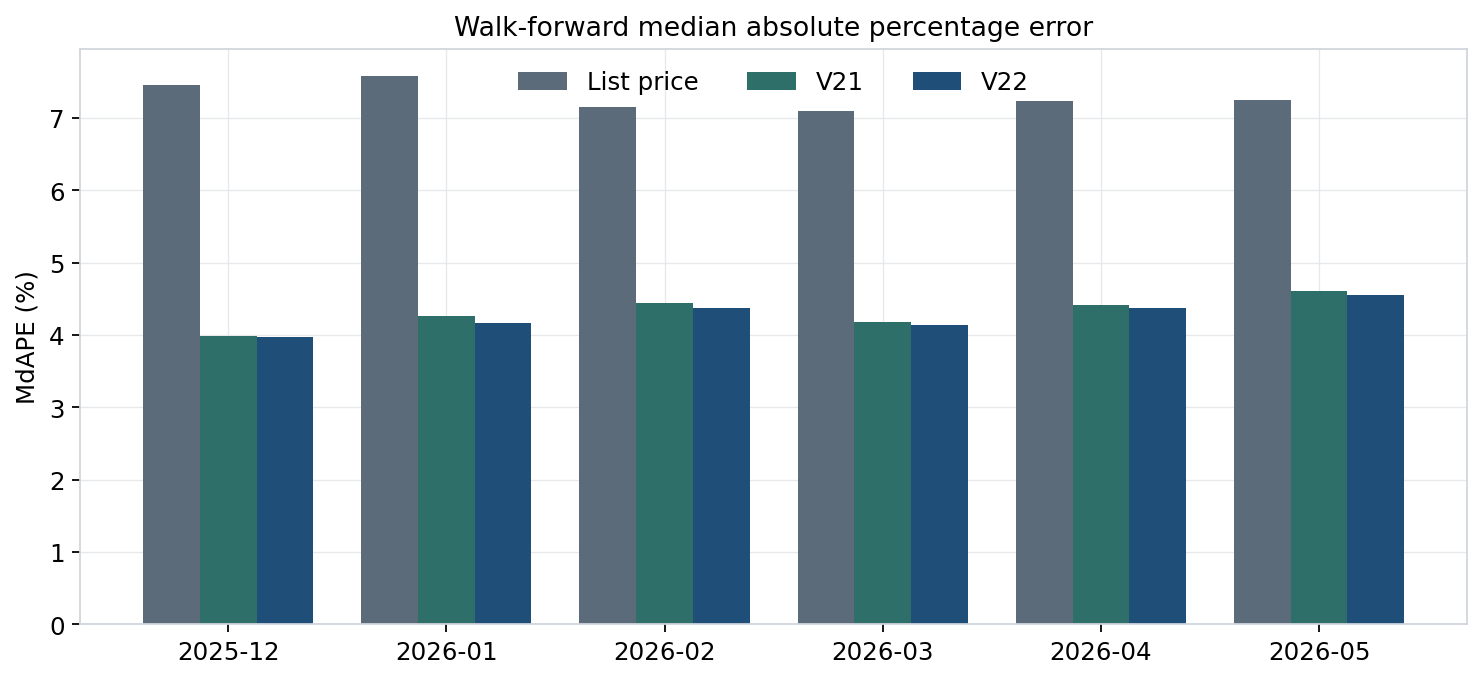
\includegraphics[width=\linewidth]{walkforward_mdape.png}
\caption{Walk-forward MdAPE by sale month. List price is the benchmark. V21 is the gap model with the recent discount and without the community category. V22 is \modelid{}.}
\label{fig:wf}
\end{figure}

\begin{center}
\small
\begin{tabular}{l r rrr rrr}
\toprule
 & & \multicolumn{3}{c}{MdAPE} & \multicolumn{3}{c}{Median signed error} \\
\cmidrule(lr){3-5} \cmidrule(lr){6-8}
Month & Homes & List & V21 & V22 & List & V21 & V22 \\
\midrule
2025-12 & 1{,}238 & 7.46 & 3.98 & 3.97 & \(+6.46\) & \(+1.22\) & \(+1.31\) \\
2026-01 & 1{,}058 & 7.58 & 4.26 & 4.16 & \(+6.60\) & \(+1.32\) & \(+1.33\) \\
2026-02 & 1{,}442 & 7.15 & 4.44 & 4.38 & \(+5.73\) & \(+0.34\) & \(+0.20\) \\
2026-03 & 1{,}816 & 7.10 & 4.18 & 4.14 & \(+5.28\) & \(+0.41\) & \(+0.46\) \\
2026-04 & 2{,}224 & 7.24 & 4.42 & 4.37 & \(+5.48\) & \(+1.35\) & \(+1.31\) \\
2026-05 & 2{,}291 & 7.25 & 4.61 & 4.55 & \(+5.12\) & \(+0.66\) & \(+0.92\) \\
\midrule
Pooled & 10{,}069 & 7.26 & 4.36 & 4.28 & \(+5.68\) & \(+0.92\) & \(+0.90\) \\
\bottomrule
\end{tabular}
\end{center}

Pooled MAPE is \(8.09\%\) for the list price, \(5.46\%\) for V21, and \(5.37\%\) for V22.

\begin{figure}[ht]
\centering
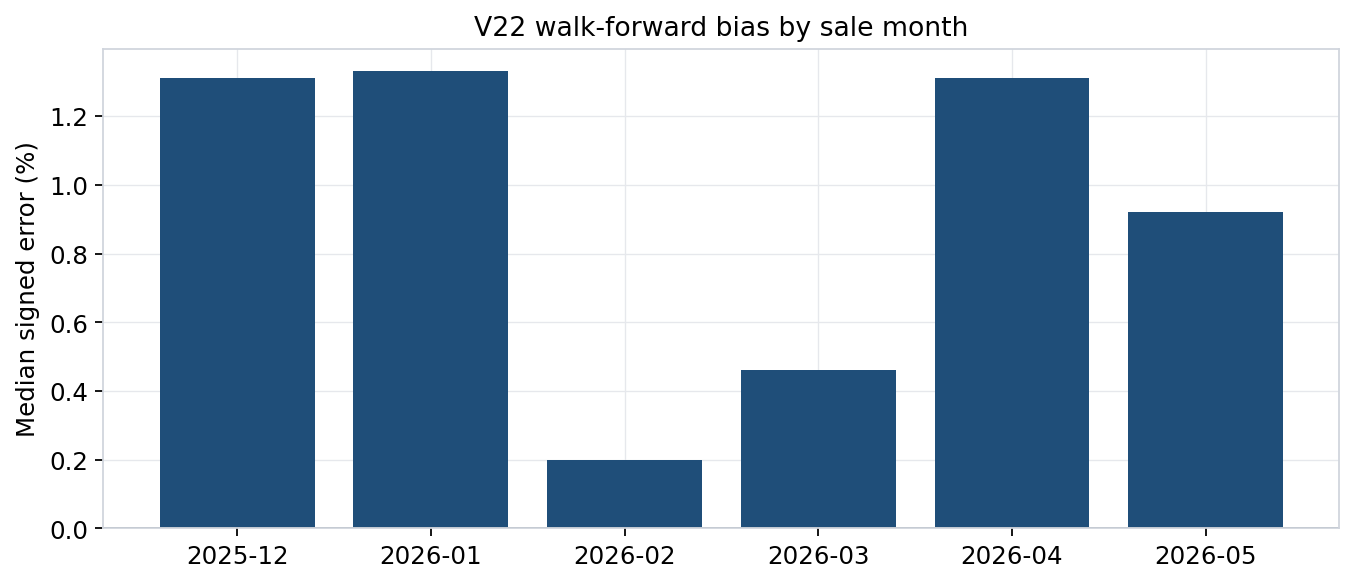
\includegraphics[width=0.92\linewidth]{walkforward_bias.png}
\caption{Walk-forward median signed percentage error of \modelid{}, by sale month. Every month is positive: the model is high, not noisy around zero.}
\label{fig:bias}
\end{figure}

\subsection{What this comparison decides}

V22 beats V21 in all six months. The margin is small, between \(0.01\) and \(0.10\) points of MdAPE, and it does not change sign. That is the right kind of evidence for a high-cardinality categorical: a large one-month win would be a suspicious leaf, and a win that flips on and off would be noise. Community stays in.

V22's pooled walk-forward MdAPE (\(4.28\)) is a little better than its developmental MdAPE (\(4.43\)). The selection process did not leave us quoting an optimistic one-shot number. Refitting every month, so that the discount tables see the latest closes, is worth about \(0.15\) points and about \(0.6\) points of median bias relative to freezing the model in November.

The monthly path is stable. V22 stays inside \(3.97\%\) to \(4.55\%\). May is the weakest month. The list-price benchmark is not weakest in May (it is weakest in January, at \(7.58\%\)), so the spring rise in model error is not only ``the market got harder for the ask.'' It is small enough that it does not overturn the specification, and it is visible enough that ongoing monitoring should plot the month, not only a half-year pool.

\subsection{Challengers under the same protocol}
\label{sec:challengers}

\begin{center}
\begin{tabular}{lrrr}
\toprule
Model & MdAPE & MAPE & Median signed \\
\midrule
Log OLS \(+\) residual forecast & 4.84 & 6.00 & \(+0.54\) \\
V13, LightGBM on log price & 4.46 & 5.63 & \(+0.86\) \\
V15, V13 plus a tuned monthly weight & 4.55 & 5.68 & \(-1.75\) \\
V19, V13 plus a 3-month level shift & 4.43 & 5.56 & \(-0.39\) \\
V21, gap \(+\) recent discount & 4.36 & 5.46 & \(+0.92\) \\
\modelid{} & 4.28 & 5.37 & \(+0.90\) \\
\bottomrule
\end{tabular}
\end{center}

V19 is the important loser. On the one-shot developmental cut it was the best number in the notebook (\(4.40\)). Walked forward, with the shift re-estimated each month from the three months before the scored month, it is \(4.43\), behind V21 and V22. Its December shift was \(+2.35\%\) and its May shift was \(+0.02\%\). A correction that changes size that fast is a description of the recent residual, not a stable property of the book. Shipping it would have meant choosing the model that won the fitting window.

V15's weight, re-chosen each month on the prior five months, ran from \(0.65\) in December down to \(0.35\) in May, and the pooled forecasts came out \(1.75\%\) low. A second-stage multiplier fit on a short, already-stale slice does not travel.

The log-linear model plus its residual forecast remains the right benchmark for ``how far can a common monthly factor get?'' Walk-forward MdAPE \(4.84\%\) against the tree's \(4.28\%\) is the cross-sectional contribution, about half a point, once time is already in the model. The larger contribution relative to the raw ask is the time adjustment itself.

\section{Error analysis}
\label{sec:errors}

Segmented errors are from the developmental refit (one origin, MdAPE \(4.43\%\)). They describe where that fit misses. They are not a second walk-forward.

\begin{figure}[ht]
\centering
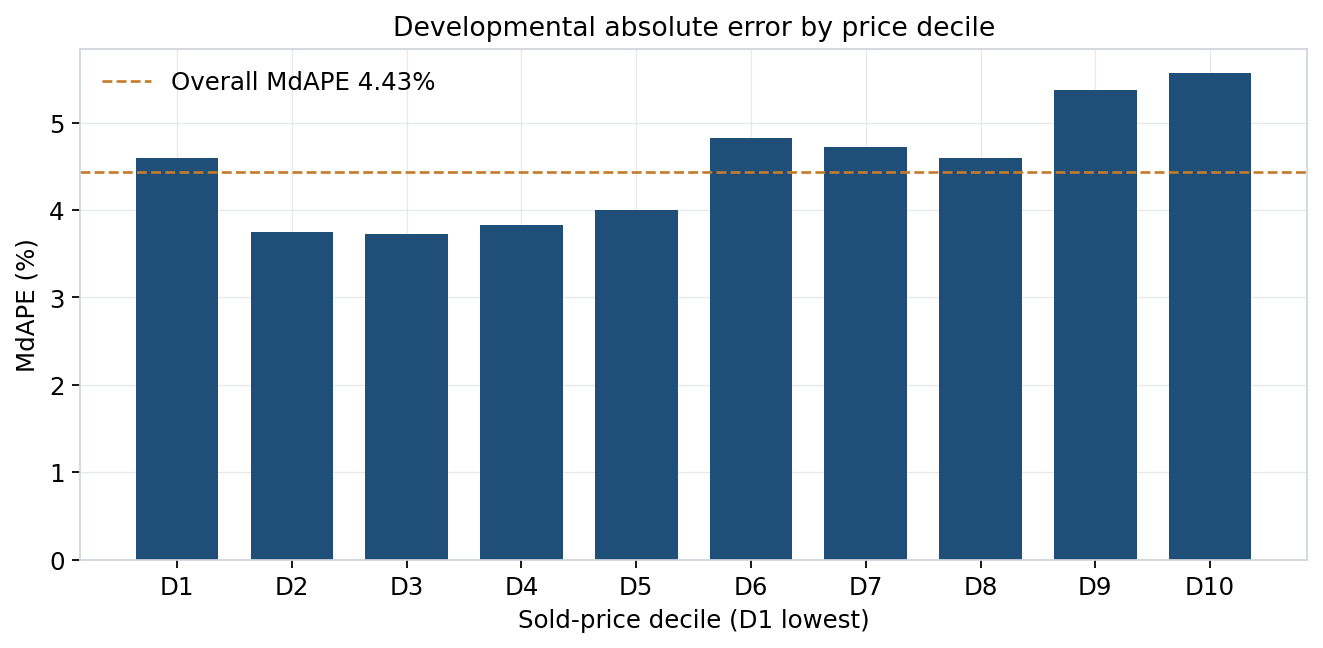
\includegraphics[width=0.92\linewidth]{error_by_decile.png}
\caption{Developmental MdAPE by sold-price decile. The dashed line is the overall \(4.43\%\).}
\label{fig:decile}
\end{figure}

\begin{center}
\small
\begin{tabular}{lrrrrr}
\toprule
Decile & Homes & Sold price, from & Sold price, to & MdAPE & Median signed \\
\midrule
D1 & 1{,}007 & 226{,}200 & 440{,}400 & 4.59 & \(+3.69\) \\
D2 & 1{,}008 & 440{,}500 & 521{,}000 & 3.75 & \(+2.07\) \\
D3 & 1{,}006 & 521{,}100 & 597{,}000 & 3.73 & \(+1.87\) \\
D4 & 1{,}007 & 597{,}100 & 692{,}000 & 3.83 & \(+1.56\) \\
D5 & 1{,}009 & 692{,}100 & 805{,}300 & 4.00 & \(+1.45\) \\
D6 & 1{,}004 & 805{,}400 & 939{,}200 & 4.82 & \(+1.16\) \\
D7 & 1{,}007 & 939{,}300 & 1{,}101{,}000 & 4.72 & \(+1.09\) \\
D8 & 1{,}007 & 1{,}101{,}100 & 1{,}316{,}300 & 4.60 & \(+0.47\) \\
D9 & 1{,}007 & 1{,}316{,}800 & 1{,}761{,}200 & 5.37 & \(-0.28\) \\
D10 & 1{,}007 & 1{,}761{,}400 & 17{,}035{,}700 & 5.57 & \(+0.49\) \\
\bottomrule
\end{tabular}
\end{center}

The middle of the condo-heavy book, roughly \(\$440{,}000\) to \(\$800{,}000\), is where the model is sharpest, with MdAPE under \(4\%\). The top decile is both wider and more expensive: MdAPE \(5.57\%\) and MAPE \(6.97\%\), on sales up to \(\$17\) million in this window. The cheap decile is accurate in the median-absolute sense and biased high by \(3.7\%\). A user who is marking the bottom of the book to this model will be systematically rich.

\begin{figure}[ht]
\centering
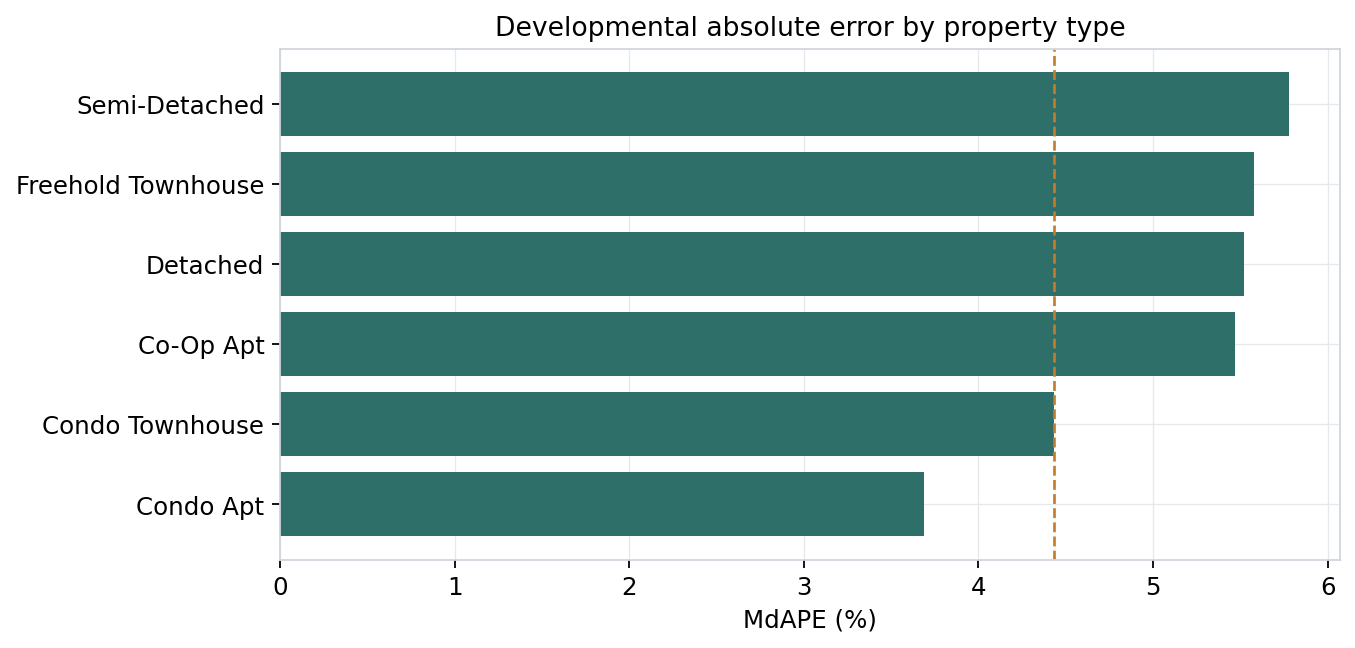
\includegraphics[width=0.88\linewidth]{error_by_type.png}
\caption{Developmental MdAPE by property type. The dashed line is the overall \(4.43\%\).}
\label{fig:type}
\end{figure}

\begin{center}
\begin{tabular}{lrrrr}
\toprule
Type & Homes & MdAPE & MAPE & Median signed \\
\midrule
Condo apartment & 4{,}843 & 3.69 & 4.36 & \(+1.65\) \\
Condo townhouse & 616 & 4.43 & 5.36 & \(+1.45\) \\
Co-op apartment & 48 & 5.47 & 6.12 & \(+3.60\) \\
Detached & 3{,}123 & 5.52 & 6.71 & \(+1.63\) \\
Freehold townhouse & 405 & 5.58 & 6.94 & \(+0.99\) \\
Semi-detached & 1{,}034 & 5.78 & 6.91 & \(-0.01\) \\
\bottomrule
\end{tabular}
\end{center}

Condo apartments are half the validation book and carry the headline. Ground-oriented homes cost about two extra points of MdAPE. Semi-detached is the weakest type and, unlike the others, is not biased high. Co-op results rest on 48 sales and should not be quoted as a type-level capital figure.

Municipalities do not separate. Developmental MdAPE runs from \(4.24\%\) in York (\(n = 124\)) to \(4.62\%\) in Scarborough (\(n = 1{,}430\)). Toronto, with \(5{,}746\) of the validation sales, sits at \(4.42\%\). The failure mode is price and structure, not the five-way municipal split. That matches the gain share: community matters, municipality does not, once community is in the model.

\begin{figure}[ht]
\centering
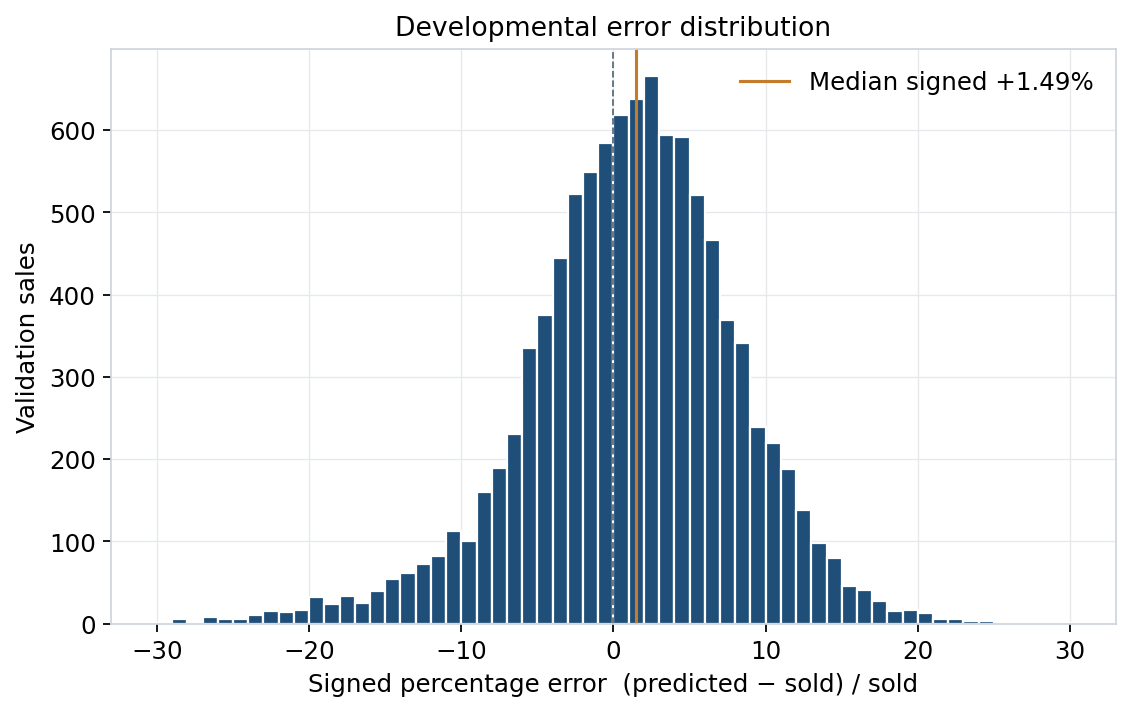
\includegraphics[width=0.86\linewidth]{error_distribution.png}
\caption{Developmental signed percentage error, truncated to the range \(-30\%\) to \(+30\%\) for display. The amber line is the median.}
\label{fig:err}
\end{figure}

The error distribution is unimodal and slightly right of zero. MAPE (\(5.53\%\)) exceeds MdAPE (\(4.43\%\)) because of the right tail of absolute errors, the same tail the 95th percentile of \(14.4\%\) describes. A service-level statement of the form ``the model is within \(5\%\)'' would be false for about half of sales. The supported statement is: the median absolute miss is about \(4.3\%\) on a one-shot half year and \(4.3\%\) walked forward, the mean absolute miss is about \(5.4\%\), and about one sale in twenty is off by \(14\%\) or more on the developmental window.

\section{Assumptions, limitations, and model risk}
\label{sec:limits}

\begin{enumerate}
\item The book is synthetic. A method that works here is evidence about this generating process. It is not a completed validation on live Toronto trades. Coordinates must not be joined to external maps.

\item The performance claim stops in May 2026. The deployment file lists homes through September 2026 and has no labels in this project. Nothing in this document is a hidden-test score.

\item The output is a point estimate. There is no interval, and the 95th percentile error above is an in-sample description of one window, not a predictive band that updates with the home.

\item Walk-forward median bias is \(+0.90\%\), and it does not change sign across the six months. Users who need a median-unbiased mark should treat the raw output as rich by about one percent, with a larger bias at low prices. An automatic haircut was tested and rejected because it was unstable.

\item \texttt{recent\_discount} is missing on \(46\%\) of developmental validation rows. The model is designed to tolerate that, through a type fallback and through LightGBM's missing-value splits. A month in which local sales dry up will lean harder on citywide features.

\item Community has 145 levels. The leaf floor of 20 rows limits how fine a community split can be. A community that is new at deployment is unseen and contributes a missing category, not a borrowed neighbour's label.

\item Hyperparameters were selected on July--November 2025 and then applied to a new target. The inner and outer feature rankings disagreed about the cumulative type discount. Both facts are reasons the walk-forward table, rather than the best developmental cell, is the claim.

\item Remarks, condition, and renovation quality are weakly present or absent. Two detached houses with the same ask, size, and community can differ by a renovation the model cannot see. That is a credible source of the extra error on ground-oriented homes.

\item The third-party AVM was excluded. If a future process can prove the estimate was known before the listing and will be present at score time, leaving it out is a limitation to revisit. Including it today would be leakage.

\item The runnable implementation is \texttt{ListAwareModel}, called from \texttt{run.py} (Section~\ref{sec:repro}). A sign-off on this document covers that entry point together with the specification and the evidence. It does not cover a separate production service. The list-price baseline remains in \texttt{models.py} and is not called.

\item No bootstrap confidence interval is reported. Resampling homes inside a month would ignore the dependence that the whole validation design exists to respect. Stability is shown by the month path instead: six months, MdAPE inside a \(0.6\)-point band, bias always positive.
\end{enumerate}

\section{Ongoing monitoring}
\label{sec:monitor}

Proposed triggers, for a book that starts publishing realized sales after go-live. They are policy thresholds for review. They were not optimised as a trading rule.

\begin{center}
\begin{tabular}{p{5.2cm}p{8.2cm}}
\toprule
Measure & Review if \\
\midrule
Monthly MdAPE & Above \(6\%\) for a month. That is still better than the ask, and it is a clear step off the \(4.0\)--\(4.6\) path seen here. \\
Monthly median signed error & Outside \(\pm 2.5\%\), or positive and rising for three months. \\
Low-price band & Median signed error above \(+5\%\) on sales under \(\$500{,}000\). \\
Discount coverage & Community-level three-month cell available for under \(10\%\) of new listings. \\
Population & Condo share or median ask moves by more than 10 percentage points relative to the estimation book. \\
\bottomrule
\end{tabular}
\end{center}

Each production score should be stored with the listing identifier, the predicted price, the list price, the model version, and the sale month the tables were built through. When the sale closes, the row can be scored without refitting. A quarterly review refits the walk-forward on the latest six closed months and compares it with the \(4.28\%\) claim. A breach of the MdAPE trigger freezes promotion of a new version until development explains the month.

Champion--challenger in production should keep the list price and V21 alongside \modelid{}. The list price is the fail-safe quote. V21 is the immediate predecessor. If V22 stops beating V21 on a rolling six-month MdAPE, the category is the first component to challenge.

\section{Reproducibility}
\label{sec:repro}

We now have two ways to rebuild \modelid{}, and they agree on the claim. The figures and the one-origin developmental fit come from the figure script. The walk-forward, including the month path in Section~\ref{sec:walk}, is what the submission code writes. That code is the model we hand in.

\subsection{Where the submission lives}

\begin{center}
\small
\begin{tabular}{p{3.5cm}p{11.2cm}}
\toprule
File & What it does for \modelid{} \\
\midrule
\texttt{data.py} & Loads \texttt{listings} and \texttt{test\_list\_aware} from Hugging Face (\texttt{Baliyang/SSU\_data\_dash}), or from the folder in \texttt{DATA\_DIR}. \texttt{hide\_answers} drops sold price, sale date, days on market, and the third-party AVM before a validation row is scored. \\
\texttt{features.py} & Columns we can read off the home: \texttt{home\_numbers} with the log list price, \texttt{lot\_area}, and \texttt{area\_is\_range}. \\
\texttt{models.py} & \texttt{ListAwareModel}. \texttt{fit} builds the peer-ask tables, the three-month discount, the market lag, and the SARIMAX residual forecast from the sales it was given, then fits LightGBM on \(\log(Y/L)\). \texttt{predict} returns list price times \(\exp(\mathrm{gap})\). \\
\texttt{run.py} & The four commands below. \texttt{make\_model("list\_aware")} is the constructor it calls. \\
\texttt{check\_submission.py} & Checks the written file: one row per test id, and a positive finite price. \\
\bottomrule
\end{tabular}
\end{center}

\texttt{ListPriceBaseline} and the starter \texttt{FeatureModel} are still in \texttt{models.py}. \texttt{run.py} does not call them. Comp columns are not built in \texttt{features.py}. They are built inside \texttt{fit}, from the training sales only, and then looked up for the home being priced. Category levels are the values seen in that same training slice. An unseen community arrives as missing.

The tree settings are the ones in Section~\ref{sec:calibration}: 127 leaves, learning rate \(0.03\), 700 trees, seed \(0\). LightGBM \(4.6.0\) is the pin in \texttt{requirements.txt}, and \texttt{statsmodels} \(0.14.6\) is what fits the SARIMAX inside \texttt{fit}. A training slice under \(8{,}000\) rows, which is only the unit test, uses a short tree of 30 trees and 15 leaves so the plumbing can be checked. Every fit behind the numbers in this document is above that cutoff.

\subsection{What we run}

From the repository root:

\begin{quote}
\texttt{py -3 run.py validate}\\
\texttt{py -3 run.py report}\\
\texttt{py -3 run.py predict}\\
\texttt{py -3 run.py check}
\end{quote}

\texttt{validate} loops December 2025 through May 2026. For each month it fits on sales that closed before that month, hides the after-sale columns, and scores the month. Both tracks are written, so the file also contains the off-market model. The list-aware rows are the ones for this document. Predicted prices are rounded to the nearest dollar. The file is \texttt{validation\_predictions.csv} under \texttt{outputs/}.

\texttt{report} scores that file. It writes a markdown report, a JSON report, a LaTeX score table, and \texttt{error\_by\_price\_range.png}. The list-aware rows in the file we scored match the V22 column of the walk-forward table: pooled MdAPE \(4.28\), MAPE \(5.37\), median signed error \(+0.90\), and the six monthly MdAPEs from \(3.97\) in December to \(4.55\) in May. V21 stays a notebook comparison. This run does not refit it.

\texttt{predict} is the file we would submit, and it is a different fit. It trains on every closed sale in \texttt{listings}, through May 2026, then scores \texttt{test\_list\_aware}. It writes \texttt{submission\_list\_aware.csv} under \texttt{submissions/}, with columns \texttt{ml\_num} and \texttt{predicted\_price}. Those homes have no sold price in this repository, so the command does not produce the performance claim. The peer tables and the residual forecast in that fit have seen the six validation months, which is what we want when the home was listed after May 2026. \texttt{check} confirms the ids and the prices before the file is handed in.

\subsection{The figure script}

The charts in this document, and the developmental \(4.43\) / \(5.53\) / \(+1.49\), come from
\begin{quote}
\texttt{py -3 model-report/reproduce\_v22\_figures.py}
\end{quote}
run from the repository root. The script refits the log-linear model, the SARIMAX, the lookup tables, and one LightGBM on sales closed before December 2025, and writes \texttt{model-report/figures} plus \texttt{v22\_diagnostics.json}. It does not call \texttt{run.py}. On 6 November 2026 that refit matched the notebook. The month path was first stored in the walk-forward cells of \texttt{list\_aware\_models.ipynb}. The \texttt{validate} run above is the check that \texttt{ListAwareModel} reproduces it.

\section{Other Information}

\appendix
\section{Full developmental ladder}
\label{app:ladder}

Every row is one fit on sales closed before December 2025, scored on December 2025--May 2026. Lower MdAPE is better. A positive median signed error means the prediction is high. This ladder is the search record. Adoption used the walk-forward table in Section~\ref{sec:walk}, which covers only the shortlisted rows.

\begin{center}
\small
\begin{tabular}{p{8.6cm}rrr}
\toprule
Specification & MdAPE & MAPE & Signed \\
\midrule
List price & 7.26 & 8.09 & \(+5.68\) \\
OLS, untransformed & 6.86 & 7.83 & \(+5.60\) \\
OLS, log scale & 7.13 & 8.05 & \(+5.95\) \\
Log OLS \(+\) residual forecast & 4.78 & 5.97 & \(+0.25\) \\
Log OLS \(+\) 2022 pulse and level shift & 4.80 & 5.98 & \(+0.41\) \\
Boosted trees, numeric & 4.83 & 5.97 & \(+1.43\) \\
Boosted trees, numeric \(+\) remarks & 4.85 & 5.98 & \(+1.66\) \\
V5 XGBoost, depth 8, lr 0.05, 400 trees & 4.69 & 5.92 & \(+1.28\) \\
V6 CatBoost, depth 6, lr 0.1, L2 3 & 4.81 & 5.97 & \(+1.32\) \\
V7 Random forest, depth 20, leaf 5 & 5.05 & 6.24 & \(+2.36\) \\
V8 XGBoost, type, style, and lot & 4.63 & 5.87 & \(+1.30\) \\
V9 XGBoost, plus peer ask & 4.53 & 5.73 & \(+1.27\) \\
V10 XGBoost, plus cumulative type discount & 4.63 & 5.78 & \(+1.53\) \\
V11 retuned XGBoost on the inner-winning set & 4.57 & 5.75 & \(+1.23\) \\
V12 LightGBM, 127 leaves, lr 0.03, 700 trees & 4.54 & 5.73 & \(+1.40\) \\
V13 LightGBM, plus listing-month factor & 4.51 & 5.68 & \(+1.16\) \\
V14 V9 plus monthly weight 0.55 & 4.49 & 5.66 & \(-1.73\) \\
V15 V12 plus monthly weight 0.55 & 4.45 & 5.62 & \(-1.60\) \\
V16 rotated coordinates & 4.52 & 5.66 & \(+1.25\) \\
V17 coordinate clusters & 4.52 & 5.66 & \(+1.25\) \\
V18 ten nearest past sales & 4.53 & 5.68 & \(+1.32\) \\
V19 recent level shift on V13 & 4.40 & 5.55 & \(-1.11\) \\
V20 LightGBM on the sold-to-list gap & 4.49 & 5.59 & \(+1.41\) \\
V21 recent community discount on the gap & 4.47 & 5.59 & \(+1.07\) \\
V22 community category on the V21 design & 4.43 & 5.53 & \(+1.49\) \\
\bottomrule
\end{tabular}
\end{center}

\noindent V11 is a useful warning in the ladder. Retuning depth, learning rate, and tree count on the inner slice, then refitting, produced a December--May MdAPE of \(4.57\%\), worse than the untuned V9 result of \(4.53\%\). A search that wins on July--November 2025 can lose on the next half year. That experience is why the LightGBM grid was kept small and why the final choice was confirmed under walk-forward.

\section{References cited in the text}

\begin{itemize}
\item Friedman, J. (2001). Greedy function approximation: a gradient boosting machine. \emph{Annals of Statistics}, 29(5), 1189--1232.
\item Ke, G., Meng, Q., Finley, T., Wang, T., Chen, W., Ma, W., Ye, Q., and Liu, T.-Y. (2017).
LightGBM: a highly efficient gradient boosting decision tree.
\emph{Advances in Neural Information Processing Systems}, 30.
\item Rosen, S. (1974). Hedonic prices and implicit markets: product differentiation in pure competition. \emph{Journal of Political Economy}, 82(1), 34--55.
\end{itemize}

The stationarity checks use the augmented Dickey--Fuller and KPSS tests, and a robust STL decomposition with a 12-month period. Walk-forward validation follows \texttt{handout.md} and \texttt{run.py}: train on the past, score the next month, and repeat.

\end{document}
